\documentclass[conference]{IEEEtran}
\usepackage{graphicx}
\usepackage{tikz}
 \usepackage{enumitem}
\usepackage[colorlinks = true, citecolor = blue]{hyperref}

% math lib
\usepackage{amsmath}
\usepackage{mathrsfs}
\usepackage{caption}
\usepackage{float}
\usepackage{afterpage}
% Adjusting caption formatting and spacing
\captionsetup{
  font=small,
  labelfont=bf,
  labelsep=period, % This changes the separator to a period instead of a colon
  skip=05pt % Adjusts the space between the figure and the caption
}

% operators
\DeclareMathOperator*{\argmax}{arg\,max}
\DeclareMathOperator*{\argmin}{arg\,min}
\newcommand\ceiling[1]{\left\lceil #1 \right\rceil}

% empty set
\usepackage{amssymb}
\let\emptyset=\varnothing

% algorithms
\usepackage{algorithm}
\usepackage{algorithmic}
\renewcommand{\algorithmicrequire}{\textbf{Input:}}
\renewcommand{\algorithmicensure}{\textbf{Output:}}

\begin{document}
% --------------------------------------------
% --------------Change HERE! -----------------
% --------------------------------------------
\def\authorone{Mrunmayee Dhapre}
\def\authortwo{Anusha Kukreja}
\def\groupid{8}
% --------------------------------------------
\title{CS258 Final Report: The RSA Problem}
\author{
    \IEEEauthorblockN{\authorone\ and \authortwo}
    \IEEEauthorblockA{
        Group \groupid
    }    
}

\maketitle
\IEEEpeerreviewmaketitle


\section{Methods: RL-based Routing}
\subsection{RL Algorithms}
\subsubsection{Deep Q Network}
Deep Q-Networks (DQN) combine deep learning with Q-learning to tackle decision-making tasks in environments with high-dimensional observation spaces.  DQNs utilize convolutional neural networks to approximate the Q-value function from visual inputs, such as pixels from video games. Innovations like experience replay and fixed Q-targets help stabilize the learning process by minimizing correlations and oscillations in data. Originally demonstrated on Atari games, the effectiveness of DQNs has extended their application to fields like robotics and autonomous systems, showcasing their broad utility in AI. In the context of resource allocation for computer networks, DQN has been used in research like \cite{dqn1} and\cite{dqn2}
\\\newline
{\textbf{Configurations of the DQN:}}

\begin{itemize}
    \item \textbf{Gamma ($\gamma$):} This parameter is as the discount factor in calculating the future discounted reward. A value of 0.999 indicates a strong preference for future rewards, nearly equivalent to immediate rewards.
    
    \item \textbf{Learning Rate (lr):} We have used three learning rates \textbf{0.1}, \textbf{0.01} \& \textbf{0.001}. This parameter determines the magnitude of adjustments made to the neural network weights during each update. A higher learning rate may accelerate learning but also risks overshooting the loss's minimum points.
    
    \item \textbf{Train Batch Size:} This specifies the number of experiences drawn from the replay buffer for network updates each time. It is set to 32, a common size in many DQN applications.
    
    \item \textbf{Neural Network Configuration:} The configuration defines the architecture of the neural network employed to approximate the Q-value function, featuring two hidden layers with 128 neurons each and ReLU activation functions.
    
    \item \textbf{Exploration Strategy:} Exploration is vital in reinforcement learning to balance exploring new actions and exploiting known rewarding ones. The EpsilonGreedy strategy begins with an \texttt{initial\_epsilon} of 1.0 (100\% random actions) and gradually diminishes to 0.1 (10\% random actions) over 10,000 timesteps, ensuring thorough exploration of the environment before beginning to exploit learned values.
\end{itemize}
\\\newline
{\textbf{Usage}}

If the DQN configuration is activated, the \texttt{algo} object represents an instance of the DQN algorithm, configured to interact with an environment registered as \texttt{netenv-v0}. This environment is generated by the \texttt{env\_creator} function using a GML file, which presumably represents a network graph, as suggested by the \texttt{gml\_path} and the class name \texttt{NetworkEnv}.
\\\newline
{\textbf{Training}}

The training process involves repeatedly executing the \texttt{algo.train()} method (in this scenario, 10 iterations), enabling the agent to engage with the environment, accumulate experiences, update the Q-network, and incrementally refine its policy towards optimal actions.
\newline


\subsubsection{PPO}
Proximal Policy Optimization (PPO) is a popular reinforcement learning algorithm that strikes a balance between sample efficiency and ease of implementation. PPO improves policy gradient methods by introducing a surrogate objective function, which optimizes the policy while keeping updates within a specified threshold to ensure stable and reliable learning. This method leverages multiple epochs of mini-batch updates using the collected data, enabling more robust policy improvements. In the computer networks domain, PPO has found applications in resource allocation tasks, where it efficiently manages bandwidth and computing resources, enhancing the overall network performance and ensuring optimal utilization of available resources in research like \cite{ppo1} and \cite{ppo2}
\\\newline
\textbf{Configuration Details}

\begin{itemize}
    \item \textbf{Gamma ($\gamma$):} This is the discount factor, set to $0.999$. It determines the importance of future rewards compared to immediate ones. A high gamma close to $1$ values future rewards nearly as much as immediate rewards, which influences the agent to consider long-term benefits.
    
    \item \textbf{Learning Rate (lr):} Set to $0.01$, this parameter controls the size of the updates to the policy. In PPO, a balance is crucial because the updates need to be big enough to improve the policy but not so large that they destabilize the training.
    
    \item \textbf{Environment (env):} The \texttt{netenv-v0} environment is likely a custom environment created for a specific purpose, in this case, using the GML file to perhaps represent a network-like scenario. This environment is where the agent will interact and learn.
    
    \item \textbf{Resources:} The configuration specifies the use of no GPUs (\texttt{num\_gpus=0}) and the basic setting for environment runners, suggesting that the training is expected to be relatively light on computational resources.
\end{itemize}



\textbf{PPO-specific Training Approach}

\begin{itemize}
    \item PPO aims to take the best of both worlds in terms of policy optimization by using a clipped surrogate objective function. This clipping moderates the updates, avoiding too large policy updates, which helps maintain stable and reliable improvement.
    
    \item It is often used in environments where the action space is either discrete or continuous and has shown great success in a wide range of scenarios.
\end{itemize}



\subsection{State Space}
A state space represents all possible states that an agent can encounter in its environment. Each state encapsulates the information needed to make decisions and predict outcomes, often defined by specific variables relevant to the task. The agent interacts with the environment by taking actions, receiving rewards, and transitioning between states, with the goal of maximizing cumulative reward.\\
In this project, the state space also captures the current node that the agent is at in the graph. The state space is implemented using the \texttt{spaces.Dict} to create a dictionary of different observation components:
\begin{itemize}
    \item \textbf{link\_utilization}: This is an array representing the utilization of each link in the network. It's defined by \texttt{spaces.Box(0, 10, shape=(len(self.graph.edges),), dtype=int)}, which specifies a bounded integer box space for each edge in the graph, with values ranging from 0 to 10.
    \item \textbf{req}: This represents the current request as an array of source and destination node indices. It’s defined by \texttt{spaces.Box(0, len(self.nodes) - 1, shape=(2,), dtype=int)}, indicating a continuous box space where each dimension corresponds to node indices.
    \item \textbf{current\_node}: This represents the agent's current location in the network as a single integer index of the current node. It’s implemented as \texttt{spaces.Discrete(len(self.nodes))}, defining a discrete space with as many possibilities as there are nodes in the graph.
\end{itemize}
% Explain state/action/reward
% Make sure you provide enough information to reconstruct results
% Check https://gymnasium.farama.org/environments/box2d/lunar_lander/ for some examples

\subsection{Action Space}

The action space is initially set to \texttt{spaces.Discrete(len(self.nodes))} but is dynamically adjusted to reflect valid actions based on the agent's current node:

\begin{itemize}
    \item \textbf{\_update\_action\_space}: This function updates the action space to reflect valid moves from the current node to its neighboring nodes. The action space is narrowed to only include indices of these neighbors, making the action space situationally specific and reducing unnecessary options.
\end{itemize}

\subsection{Reward Function}


The reward function is defined within the \texttt{step} function where the agent's actions are evaluated:
\begin{itemize}
    \item \textbf{Success Reward}: The agent receives a reward of \(+1\) if it can successfully utilize an edge to move towards the request's destination without exceeding the link’s capacity (\(\text{utilization} \leq 10\)). This rewards the agent for efficient resource utilization.
    \item \textbf{Blocking Reward}: A penalty of \(-1\) is given if the agent tries to utilize a link that is already at maximum capacity, which reflects poor decision-making or an infeasible action.
    \item \textbf{Termination and Continuation}: If the agent reaches the destination node specified in the request, or if the number of rounds equals the number of requests, the episode is terminated. Otherwise, the environment generates a new request and continues.
\end{itemize}

\section{Method: Spectrum Allocation}
The heuristic implemented in the \texttt{networkmodel.py} script revolves around dynamically allocating network resources for requests using a color mapping strategy, similar to wavelength or frequency allocation in optical or wireless networks.

\subsection{Heuristic Objective}
The primary goal of the heuristic is to efficiently map network requests (defined by source, destination, and holding time) onto a network, optimizing the use of available resources (colors or channels) on each link to minimize blocking (the inability to service a request).

\subsection{Heuristic Approach}

\subsubsection{Routing and Resource Allocation}
\begin{itemize}
    \item For each incoming request, the heuristic attempts to find a path from the source to the destination node using the shortest path algorithm.
    \item It then tries to allocate a ``color'' for the request on each link of this path. A color represents a specific channel or frequency slot available on that link.
\end{itemize}

\subsubsection{Color Allocation}
\begin{itemize}
    \item The allocation is done by checking available colors on each link along the chosen path. An available color is one that is not currently occupied by another request with non-zero holding time.
    \item If a color is available, the request is assigned to this color for each link along its route, and the holding time is recorded.
    \item If multiple  colors are available, one of the color is selected randomly and  the request is assigned to that color for each link along its route, and the holding time is recorded.
\end{itemize}

\subsubsection{Holding Time Management}
\begin{itemize}
    \item As time progresses, the holding time of each active request is decremented. Once the holding time reaches zero, the request is removed from the link, and the color becomes available again.
    \item This management ensures that colors are freed up and can be reused, which is crucial for maintaining high network utilization and low blocking rates.
\end{itemize}

\subsection{Heuristic Effectiveness}
The heuristic's effectiveness hinges on its ability to:
\begin{itemize}
    \item Efficiently find available resources (colors) along the network paths.
    \item Manage the lifecycle of each request to ensure timely release of resources.
\end{itemize}

\subsection{Challenges and Considerations}
\begin{itemize}
    \item \textbf{Blocking}: If no available colors are found on any link along the path, the request is blocked. This is a critical metric for assessing the performance of the heuristic.
    \item \textbf{Path Selection}: The choice of using the shortest path may not always be optimal, especially under high load, as it might lead to congestion on certain links.
    \item \textbf{Resource Utilization}: The approach aims to maximize the utilization of each link's capacity by managing the allocation and deallocation of colors efficiently.
\end{itemize}

This heuristic is a simplified model of more complex network resource allocation mechanisms seen in systems like optical wavelength division multiplexing (WDM) networks or wireless spectrum management, providing a useful framework for studying fundamental concepts in network resource management.
% Explain your heuristic
% If you have multiple, you can make subsections 

% If you borrow some ideas from papers, cite them with bibtex (e.g. \cite{8509143})


\section{Results}

Initially, various learning rates were applied to the algorithms. Subsequently, the learning rate that yielded the most favorable results was fixed during the simulation of the following cases:
\begin{enumerate}[label=\Roman*.]
\item All requests originate from the same source and target the same destination (\textit{San Diego Supercomputer Center} to \textit{Jon Von Neumann Center, Princeton, NJ}).
\item The source and destination nodes are chosen uniformly at random from all available nodes.
\end{enumerate}
\subsection{Learning Curve}

As described, various learning rates were employed for the DQN and PPO algorithms, specifically 0.1, 0.01, and 0.001. Figure \ref{fig:PPOresults} illustrates the results for PPO using these learning rates, while Figure \ref{fig:DQNresults} displays the outcomes for DQN.
\begin{figure}[ht]
  \centering
   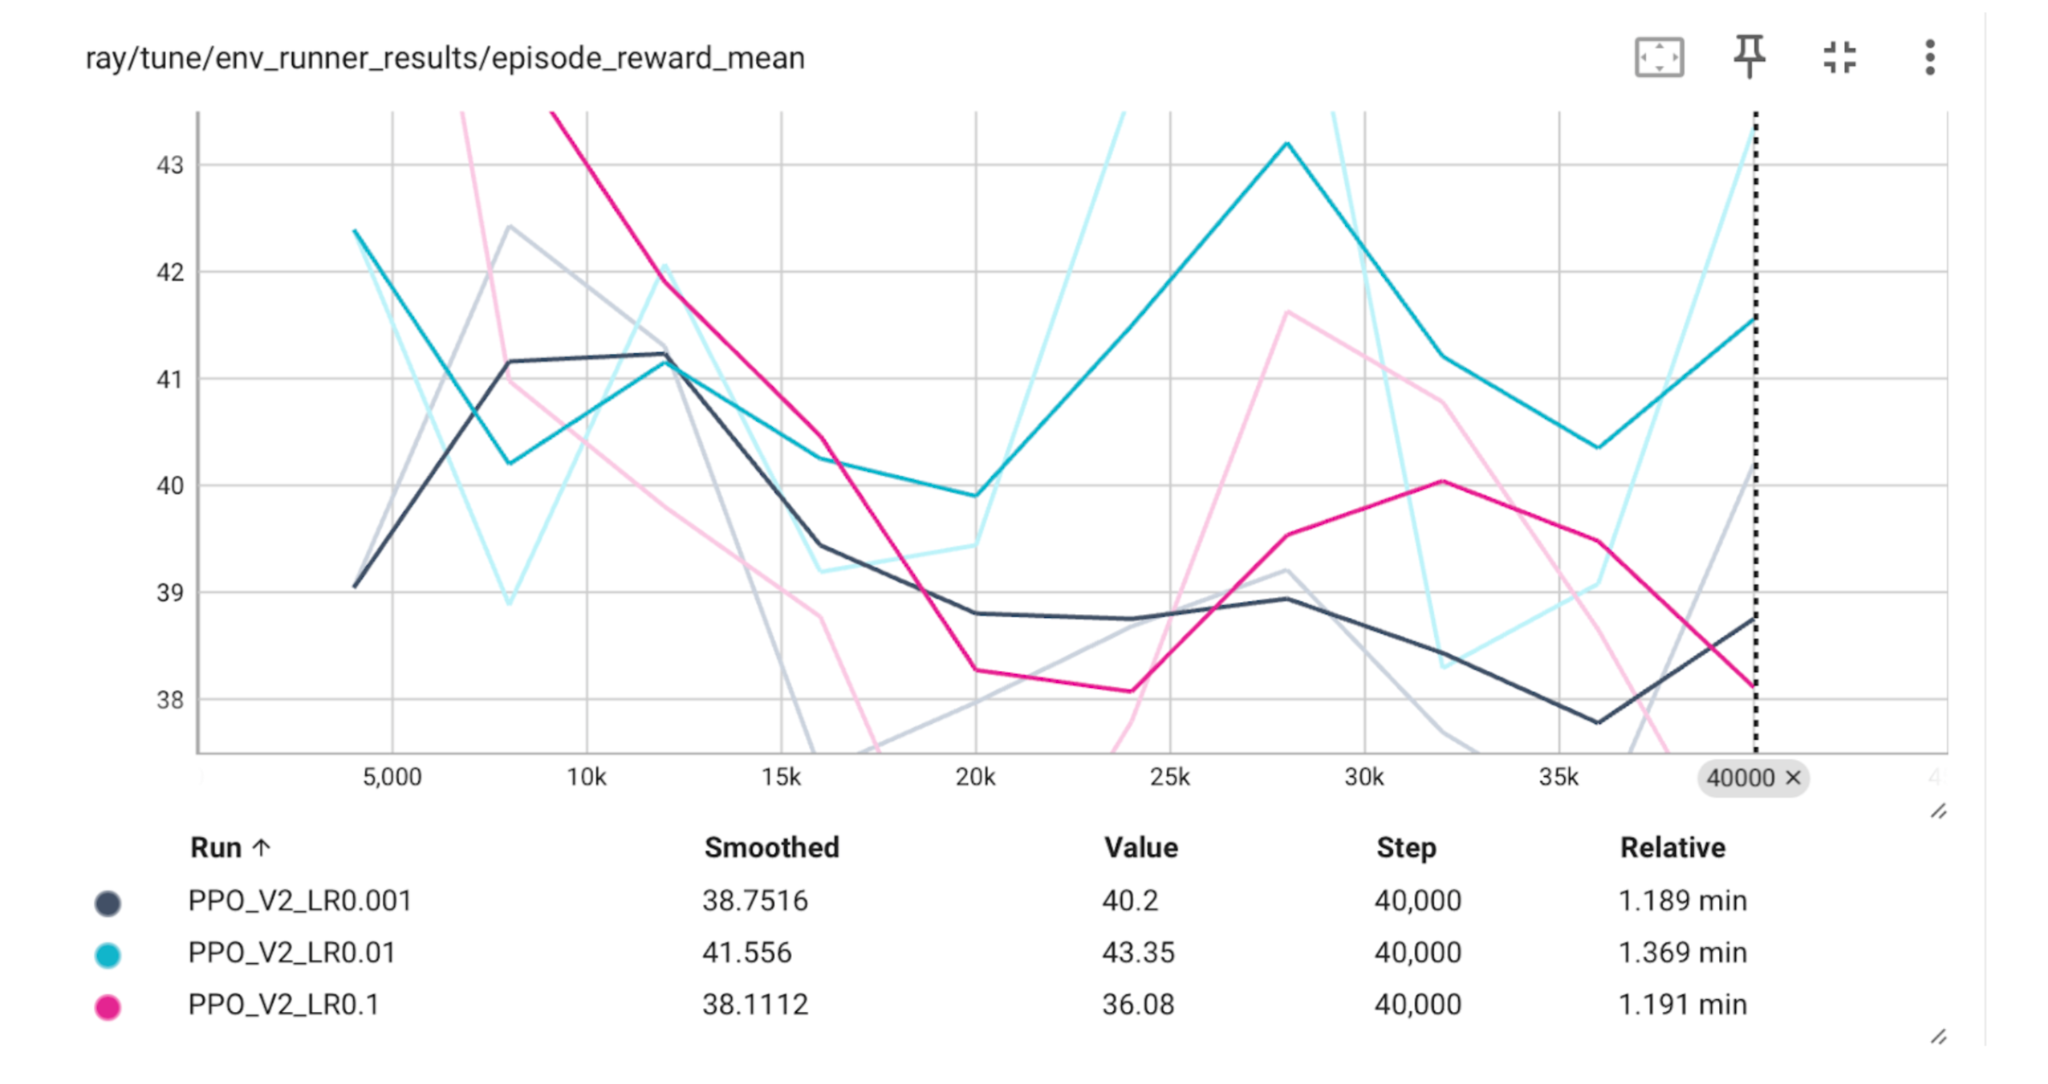
\includegraphics[width=0.5\textwidth]{PPO.png}
  \caption{Mean Reward Trend for PPO algorithm with learning rates 0.001,0.01,0.1}
  \label{fig:PPOresults}



  \centering
   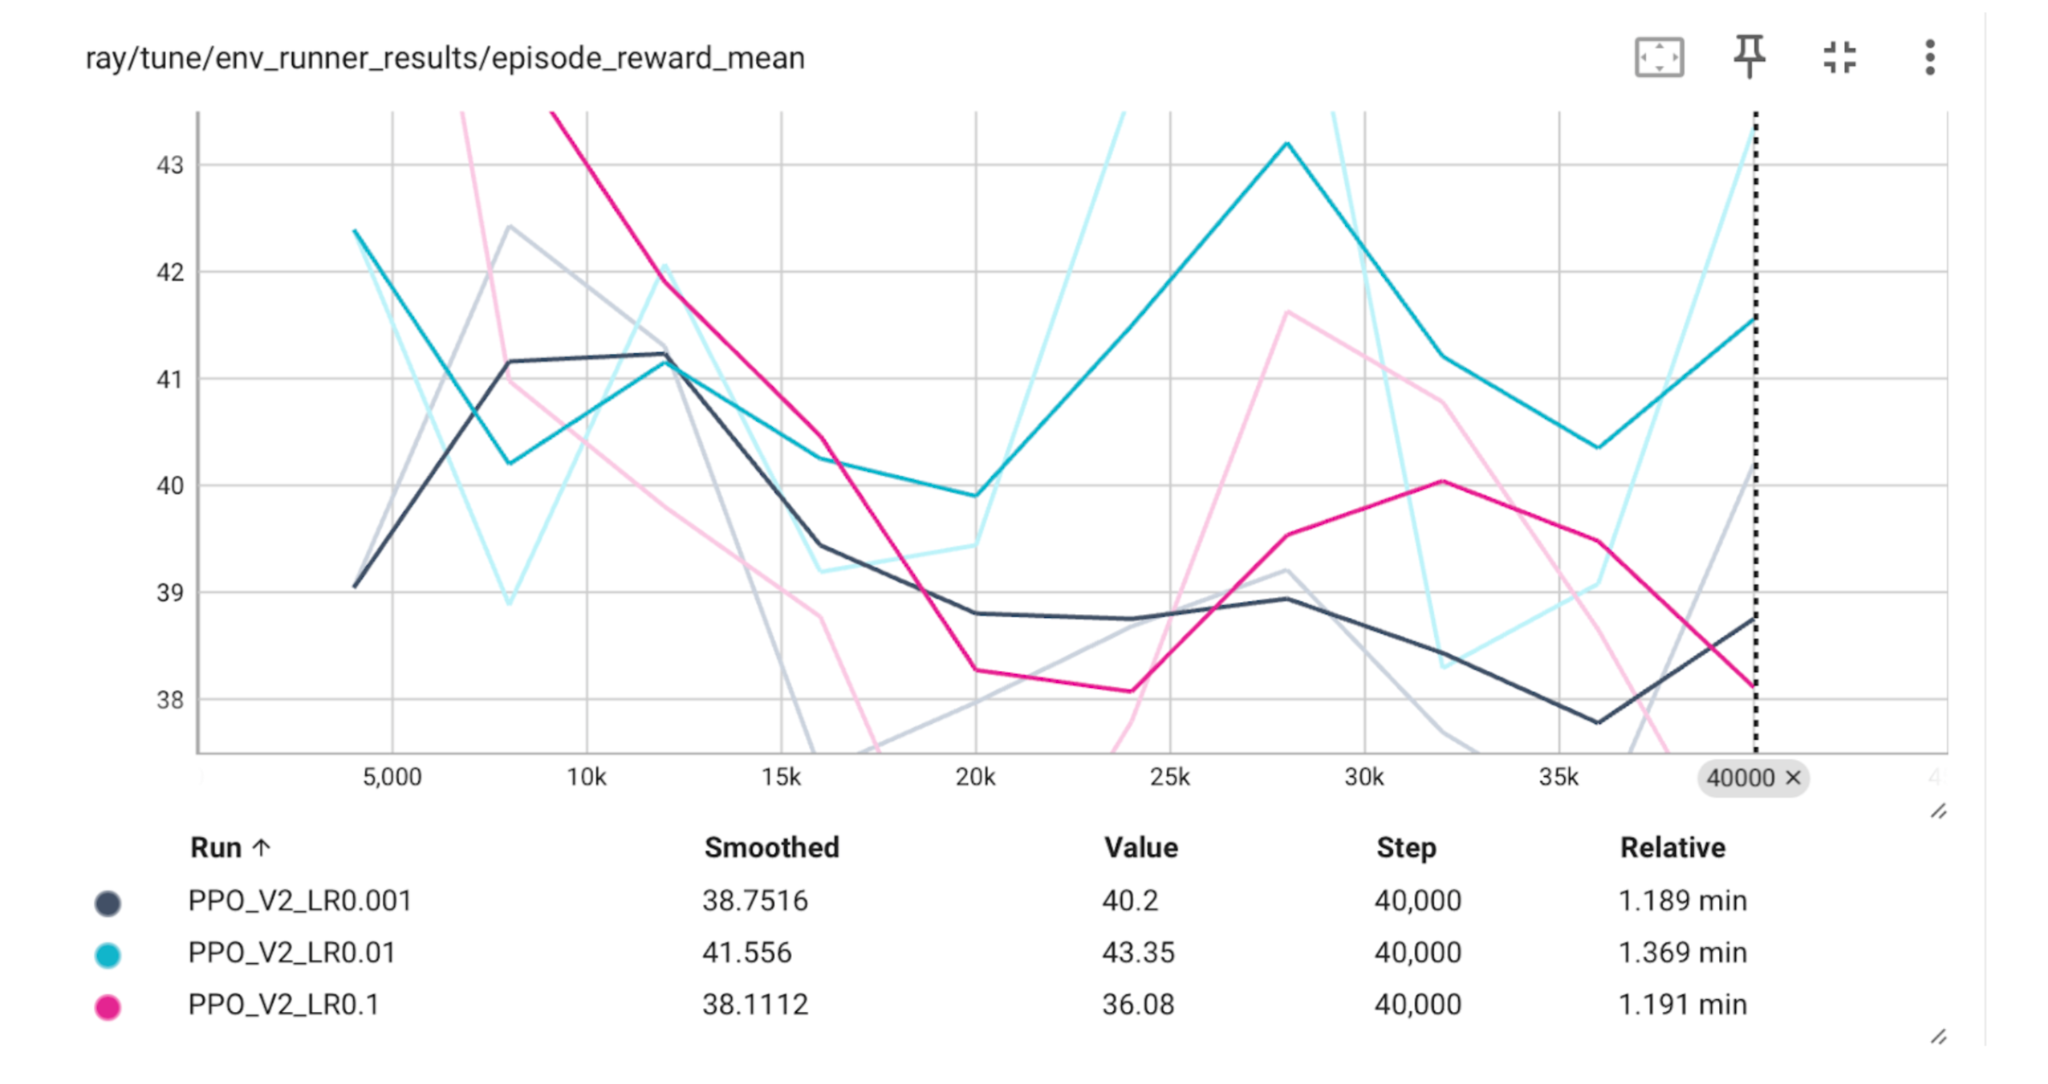
\includegraphics[width=0.5\textwidth]{PPO.png}
  \caption{Mean Reward Trend for DQN algorithm with learning rates 0.001,0.01,0.1}
  \label{fig:DQNresults}
\end{figure}

As the learning rate of 0.01 seems to be increasing over time, it was finally selected as learning rate.

% Insert figures
% Explain the results

\subsection{Utilization}

The mean utilization was computed across all network edges. Two scenarios were analyzed: fixed source and destination pairs (Case I) and randomly selected source and destination pairs (Case II). Reinforcement learning algorithms such as PPO and DQN were utilized, with training conducted over the first 100 episodes. Additionally, a heuristic algorithm was implemented and evaluated. \\
The training duration for the reinforcement learning algorithms was approximately a few minutes, and they performed quite effectively.

\begin{figure}[ht]
  \centering
   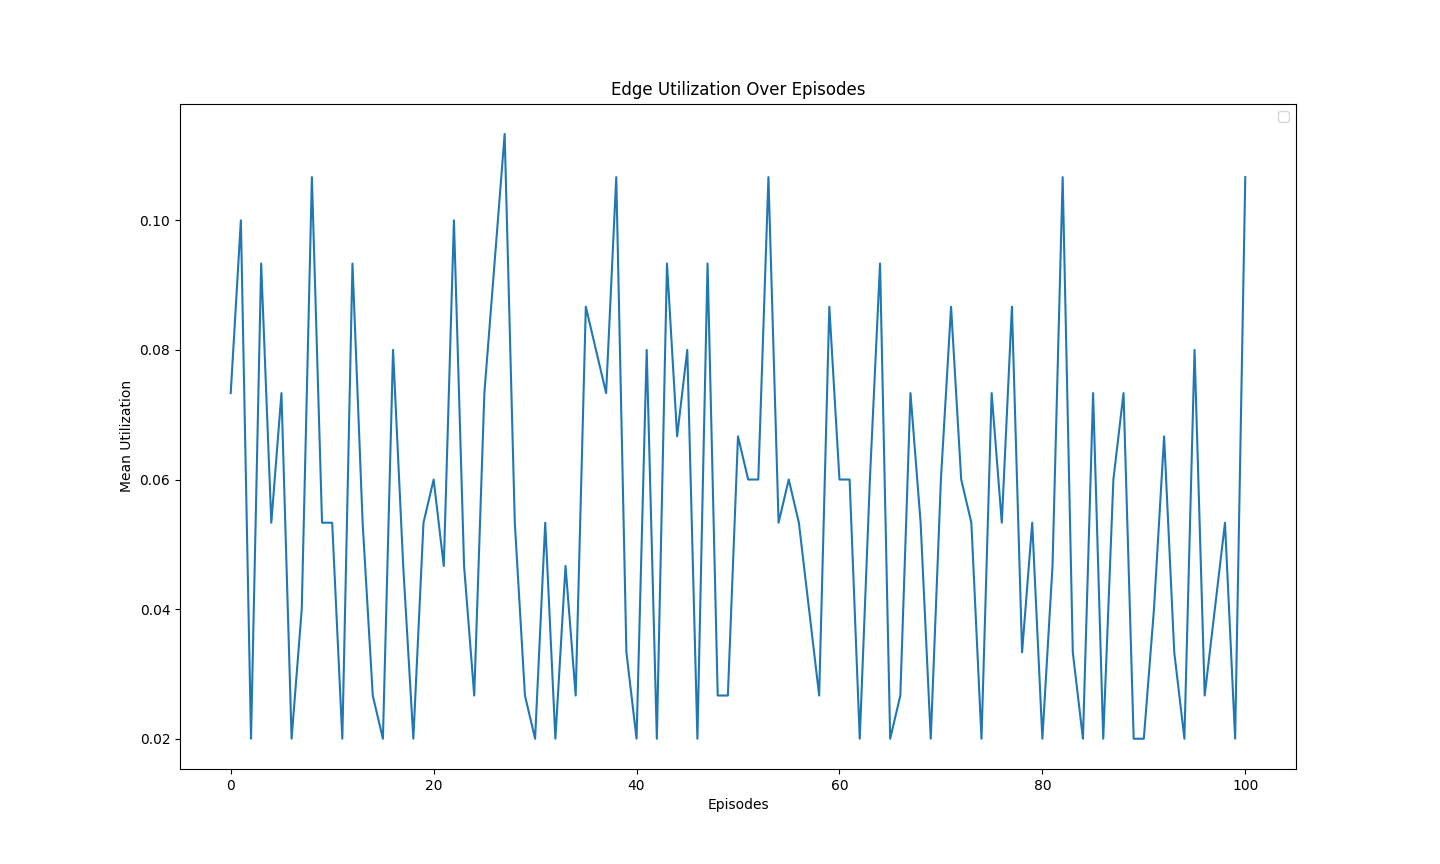
\includegraphics[width=0.5\textwidth]{util_ppo1.png}
  \caption{Mean utilization of edges with PPO algorithm - Case I}
  \label{fig:util_ppo1}
\end{figure}

\begin{figure}[ht]
  \centering
   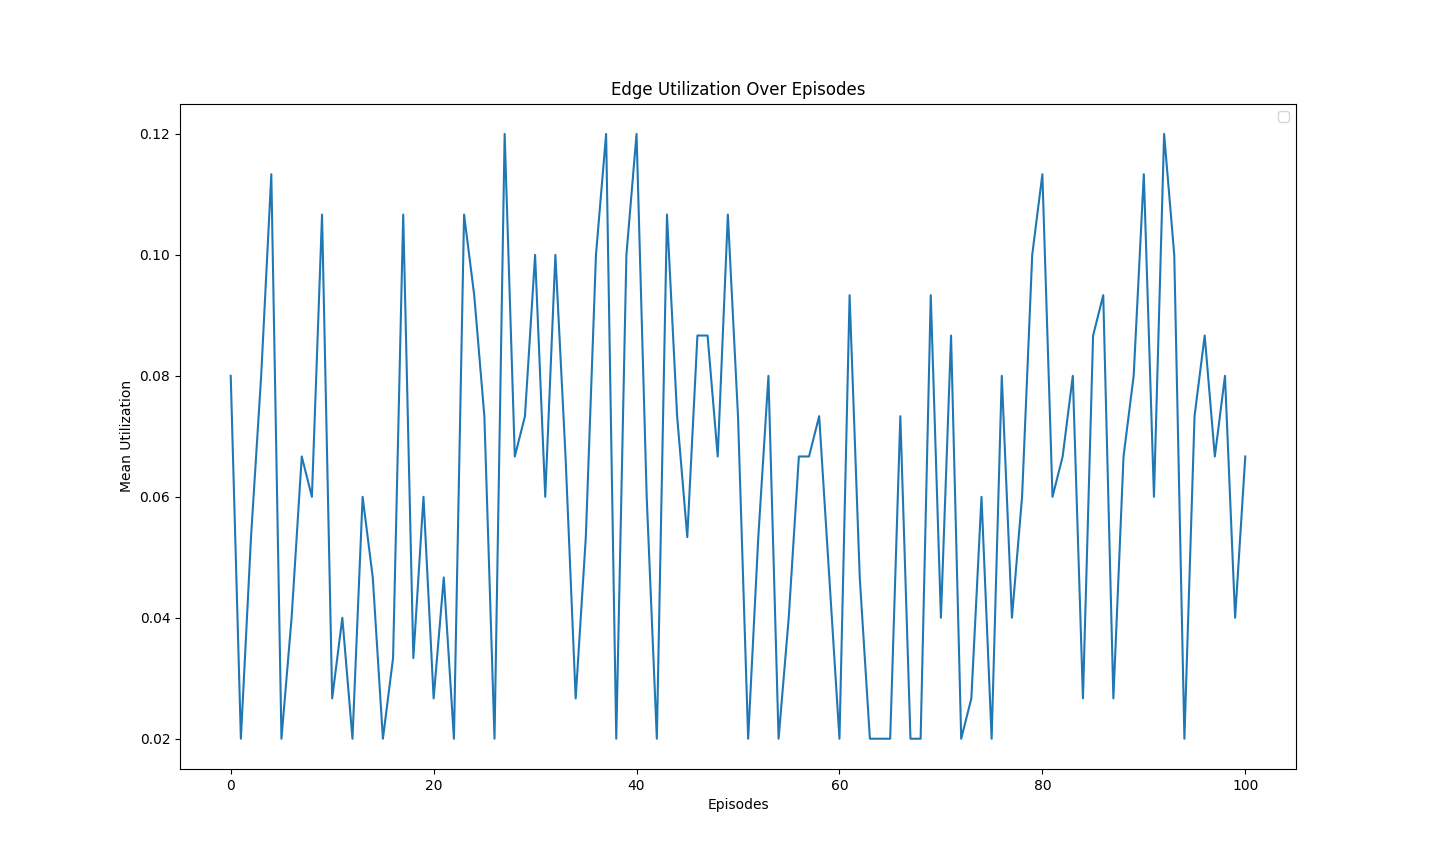
\includegraphics[width=0.5\textwidth]{util_dqn1.png}
  \caption{Mean utilization of edges with DQN algorithm - Case I}
  \label{fig:util_dqn1}
\end{figure}

\begin{figure}[ht]
  \centering
   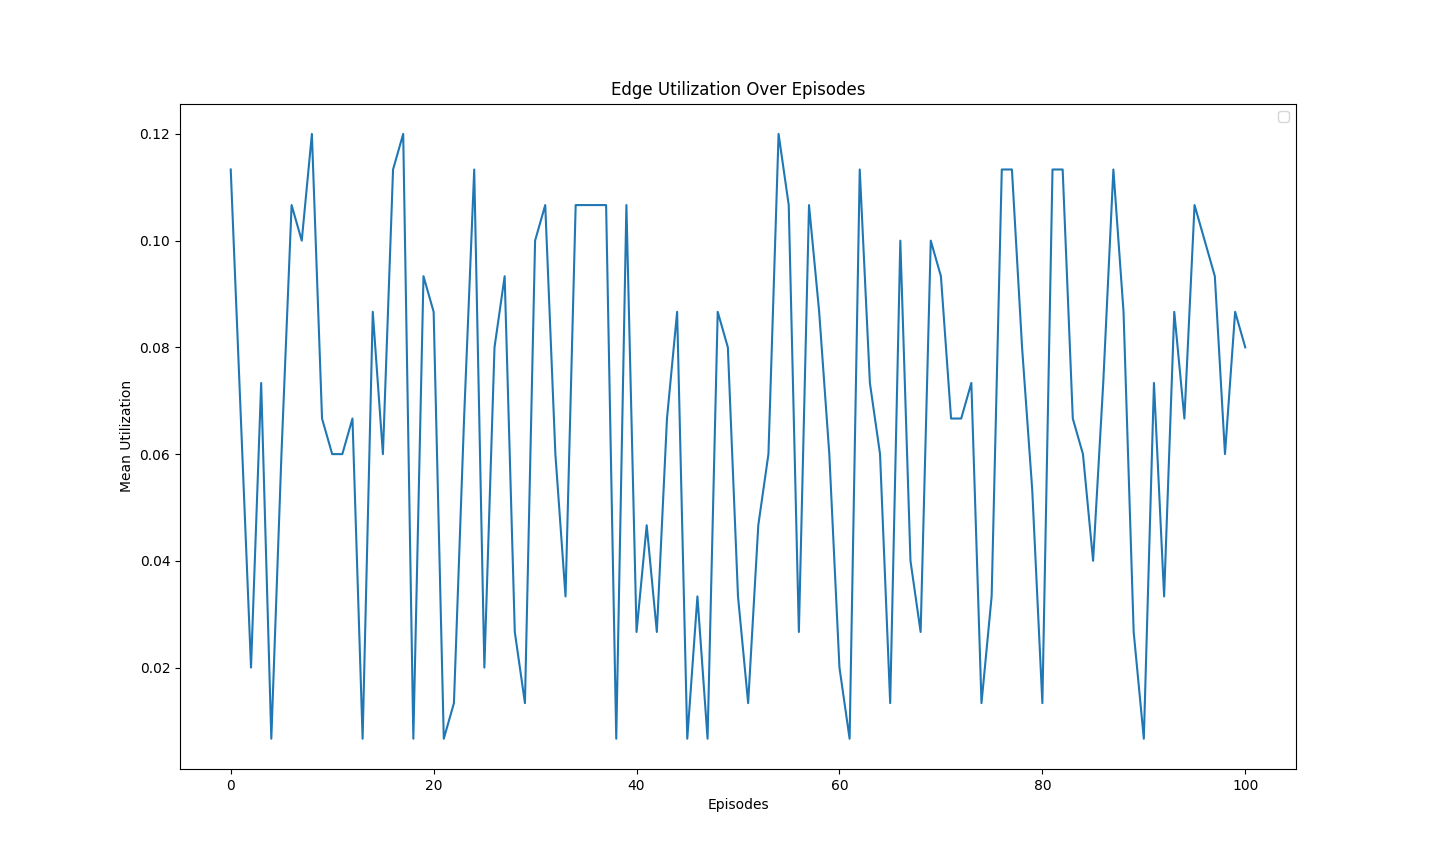
\includegraphics[width=0.5\textwidth]{util_ppo.png}
  \caption{Mean utilization of edges with PPO algorithm - Case II}
  \label{fig:util_ppo}
\end{figure}

\begin{figure}[ht]
  \centering
   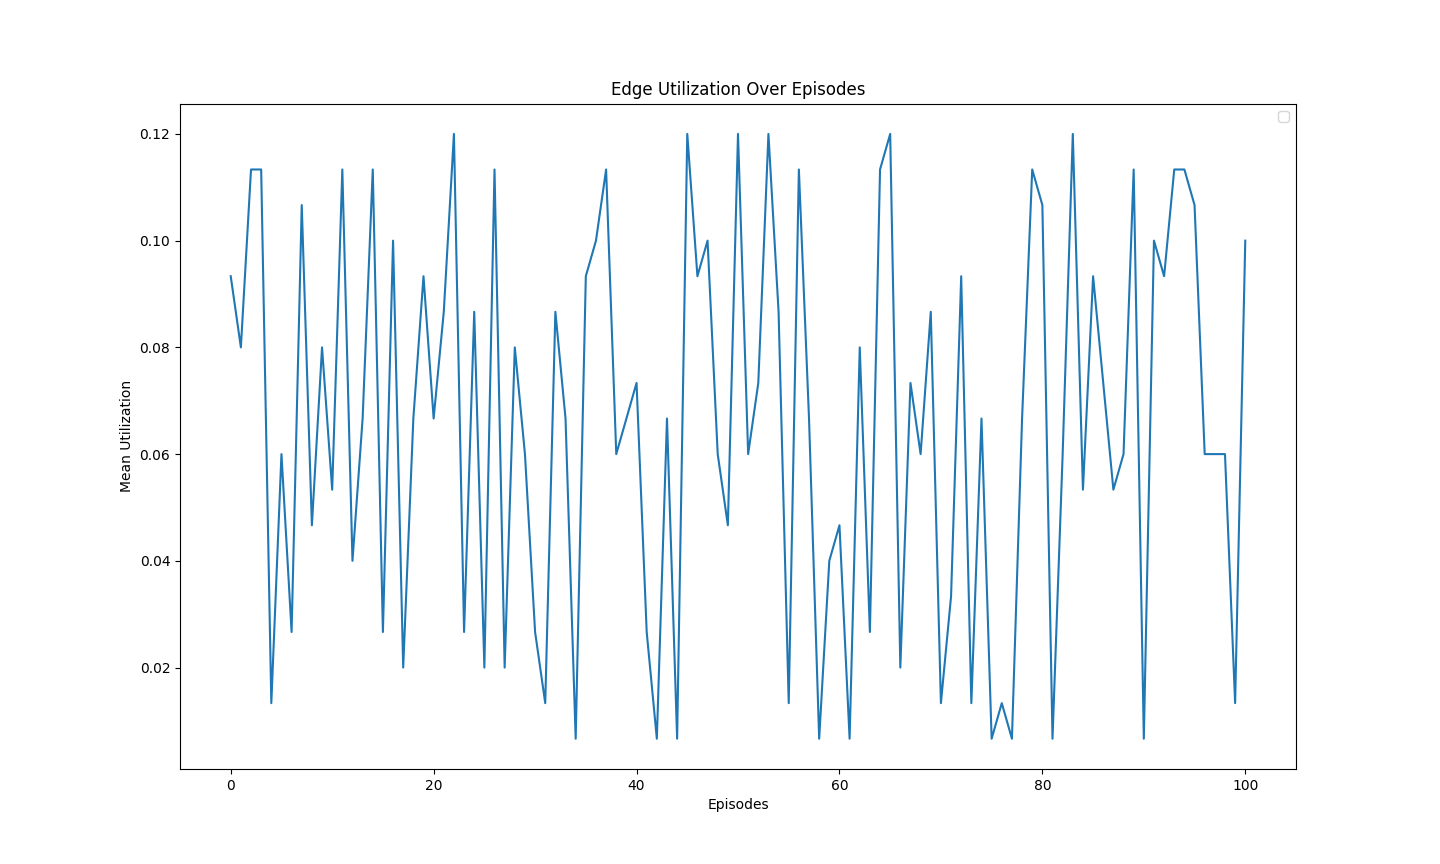
\includegraphics[width=0.5\textwidth]{util_dqn.png}
  \caption{Mean utilization of edges with DQN algorithm - Case II}
  \label{fig:util_dqn}
\end{figure}

\begin{figure}[ht]
  \centering
  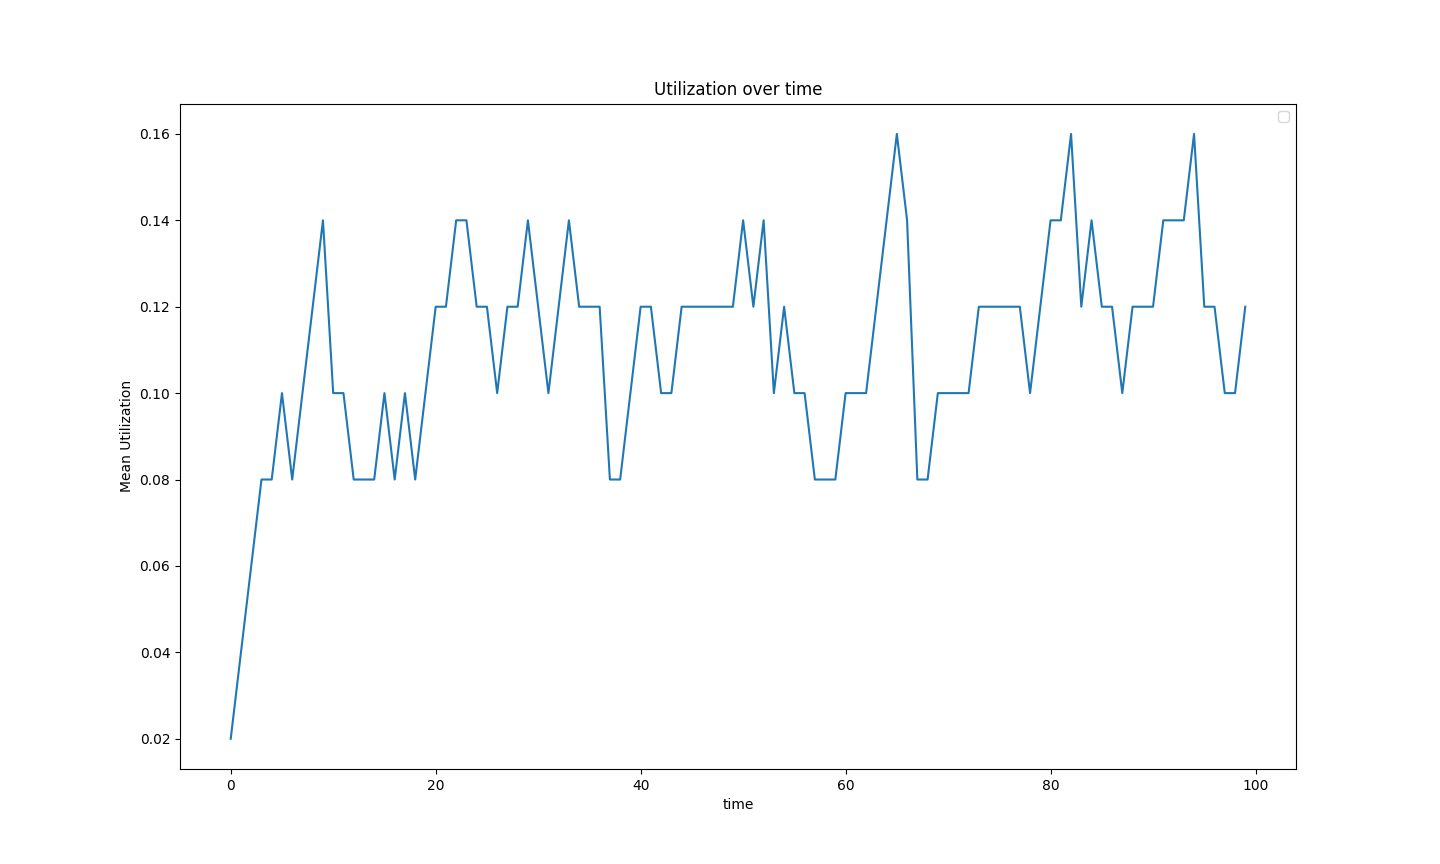
\includegraphics[width=0.5\textwidth]{util_spectrum1.png}
  \caption{Mean utilization of edges with heuristic algorithm - Case I}
  \label{fig:util_spectrum1}

  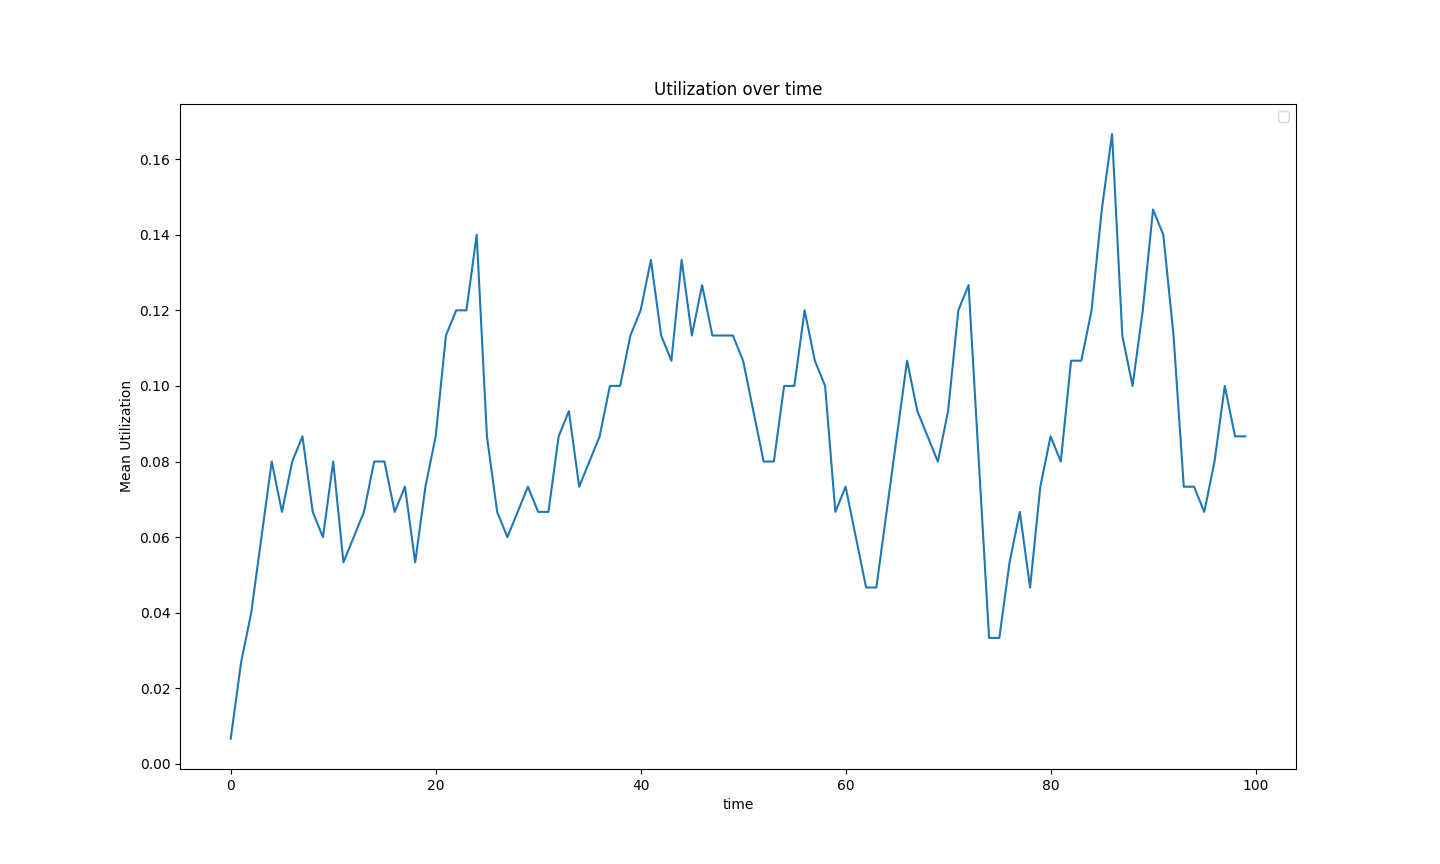
\includegraphics[width=\linewidth]{util_spectrum.png}
  \caption{Mean utilization of edges with heuristic algorithm - Case II}
  \label{fig:util_spectrum}
\end{figure}

Figures \ref{fig:util_dqn1} and \ref{fig:util_ppo1} display the utilization metrics for the DQN and PPO algorithms, respectively, in Case I, where the source and destination are predetermined. The utilization for the heuristic approach in the same scenario is presented in Figure \ref{fig:util_spectrum1}. These figures facilitate a comparison of their performances. Conversely, for Case II, where the source and destination are randomly selected, Figure \ref{fig:util_dqn} illustrates the utilization for DQN, Figure \ref{fig:util_ppo} for PPO, and Figure \ref{fig:util_spectrum} for the heuristic approach. 


\subsection{Comparison}
The results from experiments are compared and presented below.

\begin{itemize}
    \item In the first case, the utilization metrics for the heuristic approach are significantly poorer compared to the reinforcement learning approaches, indicating that reinforcement learning yields superior results. The two RL techniques, DQN and PPO, exhibit comparable performances.
    \item In the random approach (Case II), the heuristic method also under performs. In contrast, the reinforcement learning approaches demonstrate considerably better outcomes. Among the RL techniques employed, PPO appears to have a slight performance edge over DQN.
\end{itemize}


\bibliography{ref}


\bibliographystyle{ieeetr}


\end{document}



